\section{Another Way to Describe a Point: Polar Coordinates}

The Cartesian description of a point uses two signed coordinate values obtained
by orthogonal projection onto the axes:
\[
P=(x,y).
\]
This is natural when horizontal and vertical directions are important. It is not,
however, the only possible way to describe position in the plane. We may instead
ask two different questions:
\begin{enumerate}
    \item How far is the point from the origin?
    \item In which direction do we move from the origin to reach it?
\end{enumerate}

These questions lead to \emph{polar coordinates}. For a point different from the
origin, we use a pair
\[
(r,\theta),
\]
where
\[
r>0,
\qquad
0\leq \theta<2\pi.
\]
The number $r$ is the Euclidean distance from the origin, and $\theta$ is the
angle measured counterclockwise from the positive $x$-axis. The interval for the
angle is half-open: it contains $0$, but it does not contain $2\pi$. This choice
prevents the same direction from being written twice.

The origin is handled separately. In the usual non-unique polar notation every
pair $(0,\theta)$ represents the origin. In this course we choose the single
representative
\[
O=(0,0)
\]
so that every point has exactly one allowed polar pair. Thus the set of coordinate
pairs used here is
\[
\mathcal{P}
=
\{(0,0)\}
\cup
\bigl((0,\infty)\times[0,2\pi)\bigr).
\]

\begin{center}
\begin{tikzpicture}[scale=1.05]
    \draw[->] (-0.5,0) -- (4.8,0) node[right] {$x$};
    \draw[->] (0,-0.5) -- (0,3.8) node[above] {$y$};
    \coordinate (O) at (0,0);
    \coordinate (P) at (3.6,2.4);
    \draw[thick] (O) -- (P) node[midway,above left] {$r$};
    \draw[dashed] (P) -- (3.6,0);
    \draw[dashed] (P) -- (0,2.4);
    \draw (0.9,0) arc[start angle=0,end angle=33.69,radius=0.9];
    \node at (1.15,0.35) {$\theta$};
    \fill (P) circle (2pt) node[above right] {$P$};
    \fill (O) circle (1.5pt) node[below left] {$O$};
\end{tikzpicture}
\end{center}

The Cartesian and polar descriptions refer to the same point. The right triangle
in the figure gives
\[
x=r\cos\theta,
\qquad
y=r\sin\theta.
\]
Conversely, if $(x,y)\neq(0,0)$, then
\[
r=\sqrt{x^2+y^2}>0.
\]
The polar angle is the unique number $\theta\in[0,2\pi)$ satisfying
\[
\boxed{
\cos\theta=\frac{x}{r},
\qquad
\sin\theta=\frac{y}{r}
}.
\]
These two equations determine both the quadrant and the exact direction. The
single formula $\arctan(y/x)$ is insufficient because it loses quadrant
information and is undefined when $x=0$. In computation this unique angle is
usually obtained with the two-argument function $\operatorname{atan2}(y,x)$,
with a negative output shifted by $2\pi$.

\begin{examplebox}
Consider the point whose polar coordinates are
\[
(r,\theta)=\left(2,\frac{\pi}{3}\right).
\]
Its Cartesian coordinates are
\[
x=2\cos\frac{\pi}{3}=1,
\qquad
y=2\sin\frac{\pi}{3}=\sqrt{3}.
\]
Thus the same point may be written as
\[
P=\left(1,\sqrt{3}\right)
\]
in Cartesian coordinates and as
\[
P=\left(2,\frac{\pi}{3}\right)
\]
in polar coordinates.
\end{examplebox}

Polar coordinates are especially convenient when distance from the origin is the
main geometric feature. Let
\[
C_R
=
\{(x,y)\in\mathbb{R}^2:x^2+y^2=R^2\},
\qquad R>0.
\]
This is the set of all points in the Cartesian plane whose coordinates satisfy
\[
x^2+y^2=R^2.
\]
Geometrically, $C_R$ is the circle of radius $R$ centred at the origin. After
substituting
\[
x=r\cos\theta,
\qquad
y=r\sin\theta,
\]
the Cartesian condition becomes
\[
r^2\cos^2\theta+r^2\sin^2\theta=R^2.
\]
Since $\cos^2\theta+\sin^2\theta=1$, this reduces to
\[
\boxed{r=R}.
\]
In polar coordinates, the same circle is therefore represented by the set
\[
\{(R,\theta):0\leq\theta<2\pi\}.
\]

The set $C_R$ has not changed. The conditions
\[
x^2+y^2=R^2
\qquad\text{and}\qquad
r=R,
\quad 0\leq\theta<2\pi,
\]
describe the same geometric subset of the plane, but they use different
coordinates. In Cartesian coordinates we express a relation between horizontal
and vertical position. In polar coordinates we state directly that every point
of the set has the same distance from the origin.

\begin{center}
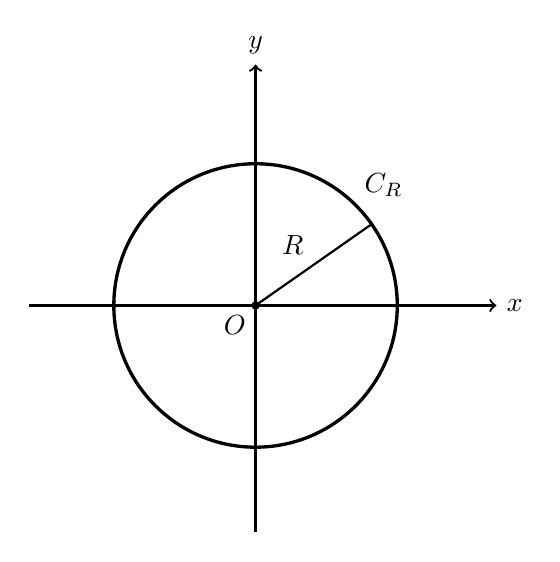
\begin{tikzpicture}[scale=0.9]
    \draw[->,thick] (-3.2,0) -- (3.4,0) node[right] {$x$};
    \draw[->,thick] (0,-3.2) -- (0,3.4) node[above] {$y$};
    \draw[very thick] (0,0) circle (2);
    \draw[thick] (0,0) -- ({2*cos(35)},{2*sin(35)})
        node[midway,above left] {$R$};
    \fill (0,0) circle (1.7pt) node[below left] {$O$};
    \node[above right] at (1.4,1.4) {$C_R$};
\end{tikzpicture}
\end{center}

\begin{remarkbox}
The restriction $0\leq\theta<2\pi$ is part of the definition used here. The
angle $2\pi$ is not included because it has the same direction as $0$. We choose
one representative angle for each direction rather than identifying the two
endpoints of the interval.
\end{remarkbox}